\section{$k$-trees}
A new family of graphs is investigated for its edge-length ratio optimization on a fixed grid. A $k$-tree is an undirected graph which is incrementally created from a $K_{k+1}$ in a way that each added vertex has exactly $k$ neighbours such that those $k+1$ vertices form a clique. Following this definition, a $4$-tree is not planar since it starts with a $K_5$. Of interest is the 2-tree and the 3-tree. 
\subsection{2-trees}
For a 2-tree, each vertex is added to exactly two neighbours, forming a clique of size 3. Starting at a $K_3$, adding a vertex will create a new face since it forms a clique. For $n$ vertices, it holds: 
\begin{align}
	|E| = 2n-3 ~~~n\geq 3
\end{align}
\begin{proof}[Proof by induction]
	\underline{IA:} $K_3$ has three edges and three vertices, $3 = 2\cdot3-3 \checkmark$\\
	\underline{IV+IS:} Suppose, the statement is true for a 2-tree $T_i$ of size $i$. Adding a vertex to $T_i$ such that $T_{i+1}$ is still a 2-tree will connect the vertex $v_{i+1}$ to two neighbours in $T_i$, increasing the edge count by two.
	\begin{align*}
		|E_{T_{i+1}}| = |E_{T_i}| + 2 = 2\cdot i -3 + 2 = 2\cdot(i+1)-3
	\end{align*}
\end{proof}
Following Euler's Formula, the amount of faces for a 2-tree of size $n$ are:
\begin{align*}
	|F|+|V|-|E| &= 2\\
	|F| &= 2 + |E| - |V| = 2 + 2n-3 - n = n-1
\end{align*}
In a planar drawing, every edge is shared by exactly two faces. So when a vertex is added to a 2-tree drawing, there are at least two faces, where the vertex can be placed. In the figure below, an example is illustrated where a vertex can be placed in more than two faces.
\begin{figure}[H]
	\centering
	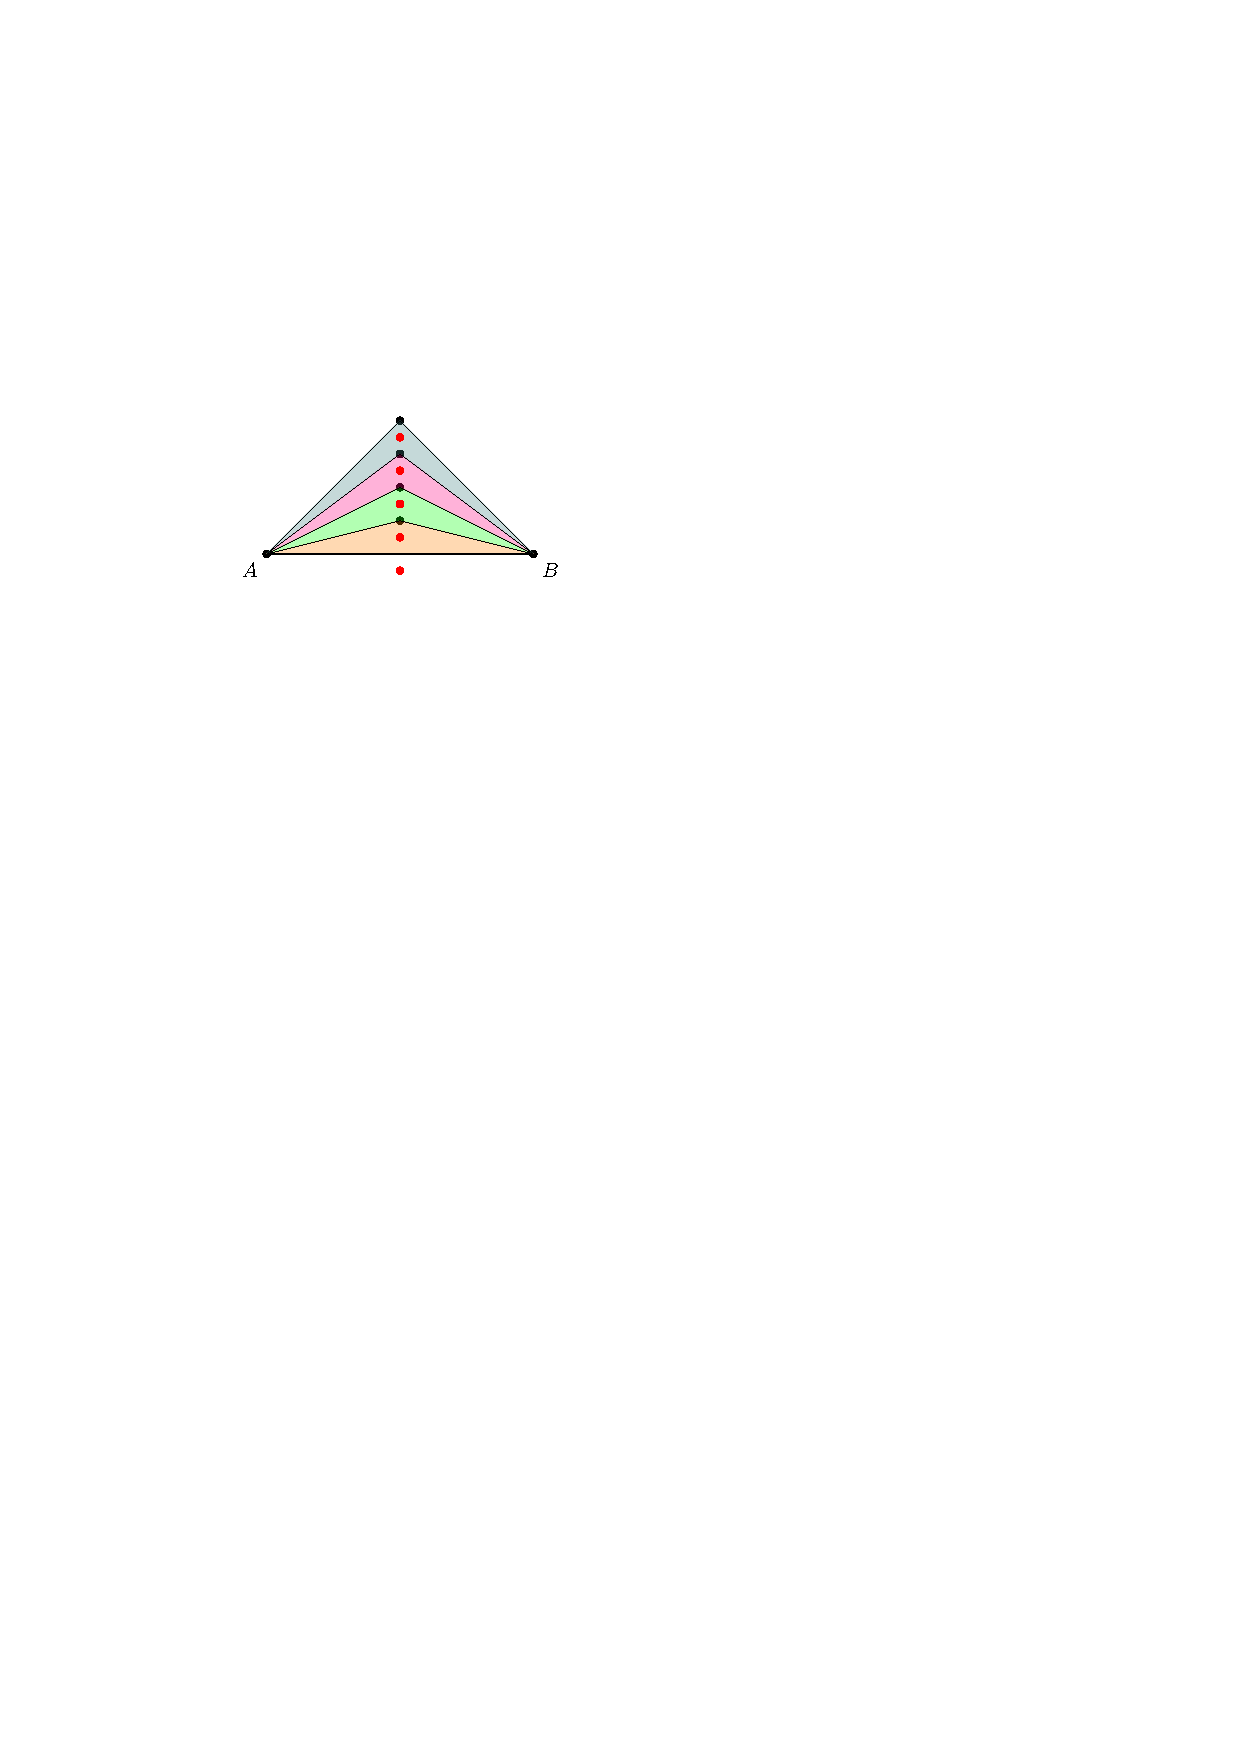
\includegraphics[width=.7\linewidth,page=1]{drawings/k-trees.pdf}
	\caption{In this drawing, a new vertex, forming a clique with A and B, could be placed in five faces, including the outerface, marked as red dot}\label{im:multiple-faces}
\end{figure}
The choice of face in which the vertex is drawn into might affect the edge-length ratio directly. One problem of a recursive drawing approach is that we do not know which problems might arise when deciding a face for a placement. So, we need a way to evaluate a suitable embedding for a given 2-tree graph.
\begin{lemma}[Expansion Lemma]
	If a graph G is $k$-connected and $G'$ is obtained by adding a vertex with at least $k$ neighbours in $G$, then $G'$ is k-connected.
\end{lemma}
\begin{proof}
	Since $G$ is $k$-connected, there are $k$ disjoint paths between every pair of vertices. Adding a vertex $v$ with $k$ neighbours will result in $k$ disjoint paths between $v$ and every other vertex of $G'$ since $G$ was already $k$-connected.
\end{proof}
\begin{theorem}
	A 2-tree is biconnected, but not necessarily triconnected.
\end{theorem}
\begin{proof}
	$K_3$ is biconnected since it is a cycle of size three. Since the 2-trees are recursively defined, adding subsequent vertices with exactly two neighbours will not harm the property of biconnectedness. In Figure \ref{im:multiple-faces}, this 2-tree serves as a counterexample for triconnectedness. A separation pair is $\{A,B\}$. Therefore, not every 2-tree is triconnected.
\end{proof}
By Spezielle Kapitel der Algorithmik Lecture about graph embeddings, the amount of embeddings for a biconnected graph is quite a lot. With $k$ parallel subgraphs, there are $k!$ permutations and every subgraph can be flipped additionally. Therefore, the amount of embeddings of biconnected graphs lies in $\mathcal{O}(n!2^n)$. Maybe, an SQPR Tree decomposition might help finding a \grqq good\grqq embedding regarding the edge-length ratio.\\
\subsubsection{First approach: Choice of vertex placement}
When adding a vertex, it will form a clique with pre-existing neighbours. This very edge is part of two faces. In this approach, the vertex added will be placed in the face with the larger area. The face will then be subdivided into two new faces. What happens, when the vertex is placed on the outerface?
\begin{lemma}
	Let $G$ be a drawing of a 2-tree and $v$ a vertex added to $G$ connecting to the neighbours defined by an edge on the outerface. Then, presuming, there is enough free area for it, $v$ can be placed on the outerface in a way that the edge-length ratio of $G'$ does increase derived by a rounding error of the grid.
\end{lemma}
\begin{proof}
	Let $l_{\max}$ be the length of the longest edge and $l_{\min}$ be the length of the shortest edge in the 2-tree $G$. We obtain $G'$ by adding a vertex $v$. If this vertex' neighbours are on the outerface and there is a free area box of size at least $l_{\min}\times l_{\min}$, then $v$ can be placed on the outerface with a distance between $l_{\min}$ and $l_{\max}$ to its neighbours and the edge-length ratio may increase when the edge-length ratio of $G$ was at 1. In this case, the placement of $v$ might not be possible to achieve edge lengths of $l_{\max}$. There will be a rounding error, depending on the granularity of the grid.
\end{proof}
So, placing vertices on the outerface will not increase the edge-length ratio significantly, presuming, there is enough free area to do so. This should work with any arbitrary number of bends per edge.\\
Now, we will investigate how the edge-length ratio behaves when a vertex is placed inside of a face. We will start with a drawing of a $K_3$, one bend allowed. We place a vertex inside of the $K_3$, creating new edges. Then, we will recursively add vertices to an edge which was created by the previous addition. The following algorithm will draw this special 2-tree:\\
\begin{algorithm}[H]
	\KwIn{$\Gamma$: Drawing of a $K_3$, $V_{\text{add}}=\{(v_i,e_i)\}$ vertices added and $|V_{\text{add}}| = m$}
	\KwOut{Drawing of a 2-tree with $m+3$ vertices}
	InsertVertex($v$,$e$) $= \{$\\
	~~~~Choose the face adjacent to $e$ with the larger area except for the outerface\\
	~~~~Place the vertex and the edges with bends in this face in a way that the face is subdivided evenly in area\\
	$\}$
	\While{$V_{\text{add}}\neq \emptyset$}{
		\For{$i \in [1..|V_{\text{add}}| = m]$}{
		\If{$e_i$.drawnIn$\Gamma$}{
		InsertVertex($v_i$,$e_i$)\\
		$V_{\text{add}} \gets V_{\text{add}}\setminus\{(v_i,e_i)\}$
		}	
	}
}
\end{algorithm}
In the special case described above, the set $V_{\text{add}}$ is initialized as follows:
\begin{align*}
	(v_1,e_1)\in V_{\text{add}}~~~e_1\text{ arbitrary edge of }K_3\\
	(v_i,e_i)\in V_{\text{add}}~~~e_i\text{ edge created by inserting }v_{i-1}\\	
\end{align*}
In this special case, the runtime of the algorithm above is in linear time. It is of interest, how the edge-length ratio will behave. In the following figures, vertex and bend placements were done intuitively.
\begin{figure}[H]
	\centering
	\begin{subfigure}{0.4\textwidth}
		\centering
		\includegraphics[width=.7\linewidth,page=2]{drawings/k-trees.pdf}
		\caption{Start with a $K_3$}
	\end{subfigure}
\begin{subfigure}{0.4\textwidth}
	\centering
	\includegraphics[width=.7\linewidth,page=3]{drawings/k-trees.pdf}
	\caption{Insert $v_1$ to neighbours $A$ and $B$}
\end{subfigure}
\begin{subfigure}{0.4\textwidth}
	\centering
	\includegraphics[width=.7\linewidth,page=4]{drawings/k-trees.pdf}
	\caption{Insert $v_2$ to neighbours $A$ and $v_1$}
\end{subfigure}
\begin{subfigure}{0.4\textwidth}
	\centering
	\includegraphics[width=.7\linewidth,page=5]{drawings/k-trees.pdf}
	\caption{Insert $v_3$ to neighbours $v_1$ and $v_2$}
\end{subfigure}
\begin{subfigure}{0.4\textwidth}
\centering
\includegraphics[width=.7\linewidth,page=6]{drawings/k-trees.pdf}
\caption{Insert $v_4$ to neighbours $v_2$ and $v_3$}
\end{subfigure}
\begin{subfigure}{0.4\textwidth}
	\centering
	\includegraphics[width=.7\linewidth,page=7]{drawings/k-trees.pdf}
	\caption{Insert $v_5$ to neighbours $v_3$ and $v_4$}
\end{subfigure}

\begin{subfigure}{0.4\textwidth}
	\centering
	\includegraphics[width=.7\linewidth,page=8]{drawings/k-trees.pdf}
	\caption{Insert $v_6$ to neighbours $v_4$ and $v_5$}
\end{subfigure}
\caption{Example of a nested drawing with one bend per edge, edge-length ratio in $\mathcal{O}(2^n)$}
\end{figure}
The edge-length ratio worsens with every inserted vertex. The shortest edge created by the $i$-th insertion has $\approx \frac{3}{4}$ length of the previous shortest edge. Therefore, the edge-length ratio in the $i$-th insertion values $\left(\frac{4}{3}\right)^i$. For $n$ vertices, the edge-length ratio of a 2-tree lies in $\mathcal{O}(2^n)$ in the worst case with this approach and one bend allowed per edge. Note, that it was not allowed to draw on the outerface.
\begin{observation}
	If it is allowed to draw on the outerface, then the above example can be drawn with an edge-length ratio of approximately 1. The edge-length ratio does not rise for an added vertex significantly, when allowing two bends per edge.
\end{observation}
\begin{figure}[H]

		\centering
		\includegraphics[width=.4\linewidth,page=14]{drawings/k-trees.pdf}
		\caption{Insert $v_i$ to neighbours $v_{i-1}$ and $v_{i-2}$, outerface allowed}

\end{figure}
There are edges which worsen the edge-length ratio, since a bend placement is not possible to maintain the uniform polyline edge-length without violating the planarity. In this example, this refers to the edges $(v_1,v_3)$, $(v_3,v_5)$ and $(v_4,v_6)$. Point of interest is, when does the special case of inserting a vertex in a face apply? In the following alternation of the example, we can observe where this case applies.
\begin{figure}[H]
	\centering
	\begin{subfigure}{0.7\textwidth}
		\centering
		\includegraphics[width=.7\linewidth,page=15]{drawings/k-trees.pdf}
		\caption{Vertex $r$ added to $A$ and $v_1$ on the outerface, since the area is bigger than the face defined by $A,B,v_1$}
	\end{subfigure}
\begin{subfigure}{0.7\textwidth}
	\centering
	\includegraphics[width=.7\linewidth,page=16]{drawings/k-trees.pdf}
	\caption{Then, vertex $v_2$ is added to $v_1$ and $A$ as before. The face defined by vertices $A,B,v_1$ is larger than the other face created by the insertion of $r$}
\end{subfigure}

\begin{subfigure}{0.7\textwidth}
	\centering
	\includegraphics[width=.7\linewidth,page=17]{drawings/k-trees.pdf}
	\caption{With every insertion of vertex $v_i$, the edge-length ratio roughly doubles}
\end{subfigure}
\caption{Example where the special case applies}
\label{im:v16r-rfirst}
\end{figure}
\begin{observation}
	When drawing $v_2$ first on the outerface, the edge-length ratio does not worsen as drastically as in the figure above.
\end{observation}
\begin{figure}[H]
	\centering
	\includegraphics[width=.4\linewidth,page=18]{drawings/k-trees.pdf}
	\caption{The same graph, but with a different ordering of edges around $v_1$  (two bends allowed)}
	\label{im:ABCv16+r}
\end{figure}
The edge $(A,v_1)$ formed two cliques, one with $r$ and one with $v_2$. More cliques are adjacent to the clique formed with $v_2$ in comparison to $r$. It was a good decision to place $v_2$ on the outerface since the outerface will provide the area to draw the remaining cliques without increasing the edge-length ratio significantly. Some sort of ordering will be helpful to evaluate the properties of a drawing.\bigskip
\begin{definition}
	For a given 2-tree $G$, the edge-clique graph $EC_G$ is defined as follows:
\end{definition}
	\begin{itemize}
	\item $V(EC_G)$ consists of the edge set of $G$, namely $E(G)$ and the clique set of $G$, namely $C(G)$.
	\item For $e = (a,b) \in  E(EC_G)$, either $a \in E_G$ and $b\in C_G$ or vice versa. If $a,b$ are both in $E(G)$ or $C(G)$, then $(a,b)\notin E(EC_G)$.
	\item For a clique vertex, there are exactly three edges vertices adjacent.
	\item For an edge vertex, there are arbitrary many clique vertices adjacent.
\end{itemize}
\begin{lemma}
	For a connected 2-tree $G$, the corresponding edge clique graph $EC_G$ is a tree.
\end{lemma}
\begin{proof}
	Suppose, that $EC_G$ is not connected. Then, there are at least two vertices which are not connected by a path. This means that there is an edge or a clique in $G$ which is not connected to the rest of the graph. But $G$ is connected. Therefore, $EC_G$ is connected.\\
	Suppose, there was a cycle in $EC_G$. Then, the cycle is of even length because of the edge restriction in $EC_G$. Consider a clique vertex $c$ of the cycle. It has two paths to another clique vertex of the cycle. Since every edge and clique of $G$ is represented once in $EC_G$, this destroys the 2-tree property.
\end{proof}
The following drawing represents a $EC_G$ for the example above in Figure \ref{im:ABCv16+r}.
\begin{figure}[H]
	\centering
	\includegraphics[width=.4\linewidth,page=19]{drawings/k-trees.pdf}
	\caption{$EC_G$ for the example of Figure \ref{im:ABCv16+r}}
\end{figure}
\begin{lemma}
	Let $p$ be a path of $EC_G$, beginning at an edge vertex and ending in an edge vertex. Then, drawing the corresponding cliques only will have an edge-length ratio of $\mathcal{O}(1)$.
\end{lemma}
\begin{proof}
	Start by drawing the starting edge. Then, draw the corresponding clique. Since $p$ is a path, the next clique will be drawn on the outerface. As we have seen before, adding a vertex to the outerface does not increase the edge-length ratio significantly.
\end{proof}
\begin{observation}
	Let $p_{\max}$ be the longest path in $EC_G$. Let $\Gamma$ be the drawing of $G$ where the longest path is drawn at first. Let $\Gamma'$ be an alternate drawing where a shorter path was drawn at first. Then, it is possible that the edge-length ratio of $\Gamma'$ is worse than the ratio of $\Gamma$.
\end{observation}
Recall the example above and the drawing resulting in Figure \ref{im:v16r-rfirst}. Drawing a shorter path in the $EC_G$ first resulted in a drawing where the longer path was not drawn on the outerface. This increased the edge-length ratio significantly.
\subsection{Previous results regarding series-parallel graphs}
There are several results for small planar drawings of outerplanar and series-parallel graphs. It was shown that:
\begin{itemize}
	\item Every series-parallel graph has a visibility representation with $\mathcal{O}(n^{\frac{3}{2}})$ area
	\item Every series-parallel graph has a visibility representation with $\mathcal{O}(\Delta n\log n)$ area, where $\Delta$ is the maximum degree of the graph
	\item It was reproven that every outerplanar graph is series-parallel, therefore these results also apply for outerplanar graphs [\cite{DBLP:journals/dcg/Biedl11}: Page 2,3]
\end{itemize}
Visibility respresentations and orthogonal drawings can be converted to polyline drawings. The following relationships hold for drawing models:
\begin{description}
	\item[Visibility Representation] Vertices are boxes, edges are horizontal or vertical line segnemts. In a 1-directional visibility representation all edges are vertical line segments.
	\item[Orthogonal Box-Drawing] Vertices are axis-aligned boxes (possibly degenerated to a line segment or point) and edges are sequences of contiguous horizontal or vertical line segments. A 1-directional visibility representation is also automatically an orthogonal box-drawing. In a flat orthogonal box drawing, every vertex is a vertical line segment.
	\item[Poly-line drawing] Vertices are points, edges are sequences of contiguous straight-line segments. A transition point between two straight-line segments is called a bend. A poly-line drawing can be obtained by modifying an orthogonal box drawing in a way such that a vertex is reassigned to a point inside of the prior box and the incident edges are rerouted to this very point. Also, empty grid lines are added until every edge has length at least 2. The area consumption is asymptotically the same since the width and height is doubled at most.
	[\cite{DBLP:journals/dcg/Biedl11}: Page 5,6]
\end{description}
Since visibility representations and orthogonal box drawings can be converted to polyline drawings with asymptotically the same area, the upper bounds given for the visibility representation also hold for poly-line drawings.
\subsection{The drawing algorithm for a maximal series-parallel graph}
A 2-terminal series parallel graph with terminals $s,t$ is defined recursively.
\begin{itemize}
	\item An edge $(s,t)$ is a 2-terminal SP graph
	\item If $G_i, i=1,2$ is a 2-terminal SP graph with $s_i, t_i$, then a serial composition with $s = s_1$, $t=t_2$ and $s_2 = t_1$ is a 2-terminal SP graph
	\item If $G_i,i=1,...,k$ is a 2-terminal SP graph, then, the parallel composition unifies $s_i$ to $s$ and $t_i$ to $t$ and the resulting graph is a 2-terminal SP graph
\end{itemize}
A series-parallel graph is a graph for which every biconnected component is a 2-terminal series-parallel graph. It is maximal if no edge can be added while maintaining a simple SP graph.
The drawing algorithm which proves the area bounds creates a visibility representation of a given maximal series-parallel graph and is also defined recursively based on 2-terminal SP graphs. The maximum height of the drawing is given by a recursive formula, depending of the heights of the subgraphs. [\cite{DBLP:journals/dcg/Biedl11}: Page 6 to 11]
Concerning the edge-length ratio, the longest edge might depend on the height of the drawing while the shortest edge might be of unit length.
\begin{description}
	\item[Invariant] Vertex $s$ contains the upper right corner of the bounding box, while vertex $t$ contains the lower right corner of the bounding box. The boxes for $s$ and $t$ can be stretched to the whole width of the drawing 
	\item[Base case] the base case is the edge $(s,t)$. Simply put $s$ over $t$ and the invariant holds
	\item[Height] The height of a drawing, denoted by $h$, can be increased preserving the invariant
	\item[Inductive step] This step is for $m>1$ edges and holds two major cases: a parallel composition and a serial composition. If the composition is a parallel one, then the recursive drawings of the $k$ parallel subgraphs will be of a serial composition and vice versa.
	\begin{itemize}
		\item During the parallel composition, $2\leq k$ subgraphs will first be ordered in their number of edges $(m_i \leq m_{i-1}, i \in[1..k])$ and then recursively drawn. The subgraphs are drawn in serial since the original step is the parallel case. The heights of the subgraph drawings are adjusted and unified with a terminal $s$ and $t$ on top and bottom of the bounding box.
		\item For the serial composition, two subgraphs $H_a, H_b$ with terminals  $s,x$ and $x,t$ are recursively drawn (in parallel). Note, that $x,t$ is an edge of $H_b$ since the original graph is a maximal series-parallel one. There are two outcomes of serial placement. Either, the boxes for $x$ and $t$ share the same row on the bottom of the bounding box, being connected horizontally, or $x$ lies in an interior row and is connected to $t$ vertically
	\end{itemize}
	\item[Output] The resulting drawing is a flat orthogonal box drawing. There are no additional columns for the vertices, every vertex contains an incident vertical edge in the base case. Since no bend is created at any time, the box drawing is in fact a flat visibility representation. It was shown that the height of the drawing is bound by $\mathcal{O}(\sqrt{n})$ and there are maximal as many columns as there are edges. The resulting drawing is in area $\mathcal{O(n^{\frac{3}{2}})}$.
	\item[Runtime] Since in this recursive algorithm every edge is touched exactly once, the total runtime lies in $\mathcal{O}(m+n)$.
\end{description}
\subsection{Edge-length ratio of a maximal series-parallel graph}
In the resulting flat orthogonal drawing without any bends / visibility representation with $\mathcal{O}(n)$ width and $\mathcal{O}(\sqrt{n})$ height, the longest edge lies in $\mathcal{O}(n)$ since edges are horizontal or vertical line segments. The shortest edge is in $\mathcal{O}(1)$ in the base case.
\subsubsection{From a flat orthogonal drawing to a polyline drawing}
To transfer a flat orthogonal drawing to a polyline drawing, empty grid lines are inserted until every edge length is at of least two. For a box of a vertex $v$, replaced the box by an arbitrary grid point and insert a bend for each edge connected to $v$ for rerouting. For each vertex, a bend might be inserted, resulting in a polyline drawing with up to two bends per edge.
\begin{lemma}
	Every maximal series-parallel graph admits a polyline drawing with two bends per edge and an edge-length ratio of $\mathcal{O}(n + \sqrt{n}) = \mathcal{O}(n)$.
\end{lemma}
\begin{proof}
	In the transition, every box of vertex in the orthogonal box drawing is substituted with a dot on the grid, therefore two bends per edge. A vertex box has width at most $\mathcal{O}(n)$, like the total width. The longest vertical edge lies in $\mathcal{O}(\sqrt{n})$, is horizontally rerouted with a line segment in $\mathcal{O}(n)$. The shortest edge stays in $\mathcal{O}(1)$, therefore the total edge-length ratio lies in $\mathcal{O}(n)$.
\end{proof}
\subsection{Next steps}
\begin{description}
	\item[Improve the worst case result] If this approach is a correct one, find a way to improve the exponential worst case of the edge-length. 
	\item[Investigate 3-trees] Since 3-trees are triconnected, there is one embedding disregarding flip. How does the edge-length ratio behave? Which face would be suitable to put on the outerface?
\end{description}

% \subsection{3-trees}